\mySection{14.4 The Kruskal-Wallis Test}
%-------------- start slide -------------------------------%{{{ 14.4
\begin{frame}{The Kruskal-Wallis Test}
	\begin{itemize}
		\item[] What is the nonparametric counterpart for the one-way ANOVA?
		\bigskip
	\item[Setup] Suppose that $k\ge 2$ independent sample of size $n_1,\cdots,n_k$ are drawn from $k$
		\begin{center}
			\textcolor{yellow}{identically shaped and scaled pdfs,}\\
			\textcolor{yellow}{except for possibly different medians.}
		\end{center}
			\bigskip
		\item[] Let $\widetilde{\mu}_1,\cdots,\widetilde{\mu}_k$ be the medians.
			\bigskip
		\item[Test] $H_0:\widetilde{\mu}_1=\widetilde{\mu}_2=\cdots=\widetilde{\mu}_k$ vs. $ H_1:$ not all the $\widetilde{\mu}_i$'s are equal.
			\bigskip
		\item[Remark] This is the test for median not mean, but if pdfs are symmetric, they are the same.
	\end{itemize}
\end{frame}
%-------------- end slide -------------------------------%}}}
%-------------- start slide -------------------------------%{{{ 1
\begin{frame}[fragile]
\begin{itemize}
	\item[] \textcolor{yellow}{Kruskal-Wallis statistic $B$}
	\begin{align*}
		B= \frac{12}{n(n+1)}\sum_{j=1}^k \frac{R_{\cdot j}^2}{n_j} -3(n+1)
	\end{align*}
	where
	\begin{center}
		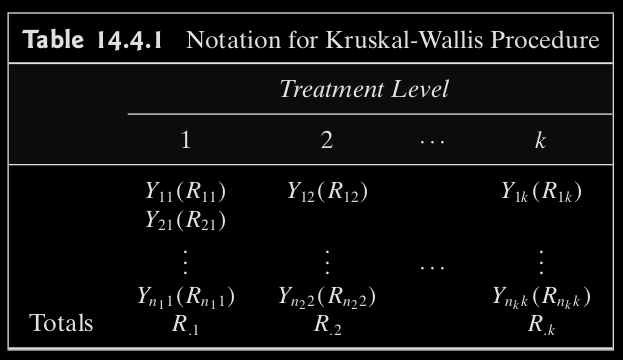
\includegraphics[scale=0.3]{Codes/Table14-4-1.png}
	\end{center}
\end{itemize}
\end{frame}
%-------------- end slide -------------------------------%}}}
%-------------- start slide -------------------------------%{{{ 1
\begin{frame}[fragile]
\begin{itemize}
	\item[Theorem] Under the above setup and under $H_0$, then
	\begin{align*}
		B= \frac{12}{n(n+1)}\sum_{j=1}^k \frac{R_{\cdot j}^2}{n_j} -3(n+1) \quad \stackrel{approx}{\sim}\quad \chi^2_{k-1}.
	\end{align*}
	\bigskip
	\item[] $H_0$ should be rejected at the $\alpha$ level of significance if  $b>\chi^2_{1-\alpha,k-1}$.
\end{itemize}
\end{frame}
%-------------- end slide -------------------------------%}}}
%-------------- start slide -------------------------------%{{{ 1
\begin{frame}[fragile]
\begin{itemize}
	\item[E.g.] Lottery over the year 1969; Whether lottery is random?
	\begin{center}
	Test if $H_0:\widetilde{\mu}_{\text{Jan}} = \widetilde{\mu}_{\text{Feb}} = \cdots = \widetilde{\mu}_{\text{Dec}}$	at $\alpha=0.01$
	\bigskip

	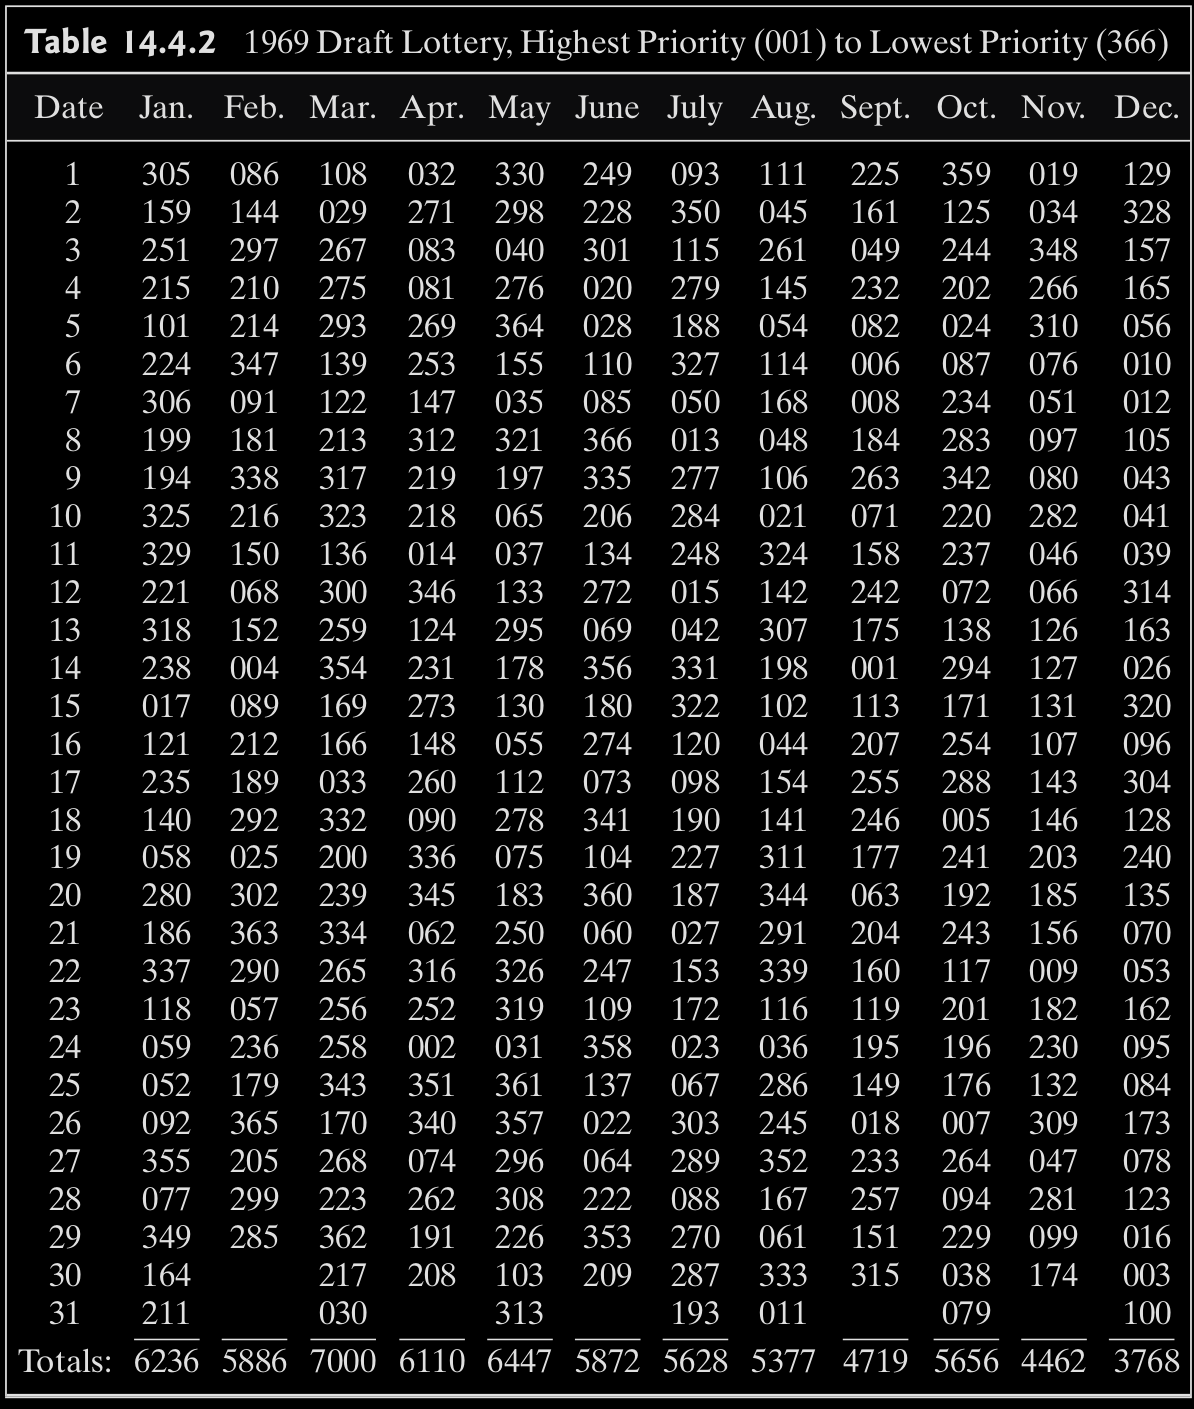
\includegraphics[scale=0.16]{Codes/Table14-4-2.png}
	\end{center}
\end{itemize}
\end{frame}
%-------------- end slide -------------------------------%}}}
%-------------- start slide -------------------------------%{{{ 1
\begin{frame}[fragile]
\begin{itemize}
	\item[Sol.] Rank the lottery for the year (see the previous table).
	\bigskip
	\item[] Compute $b$ using the formula:
	 \begin{align*}
		b & =\frac{12}{366\times 367}\left[\frac{6236^2}{31}+ \frac{5886^2}{29} + \cdots + \frac{3768^2}{31}\right] -3 \times 367\\
      & = 25.95.
	\end{align*}
	\item[] Critical region is $C=\left\{b: b\ge \chi_{0.99,11}^2 = 24.725\right\}$.
	\bigskip
	\item[] Conclusion: Reject (Lottery is {\it NOT} random). \myQED
\end{itemize}
\end{frame}
%-------------- end slide -------------------------------%}}}
